%\documentstyle[a4j,epsbox,graphicx]{jarticle}
\documentclass[a4j]{jarticle}%変更禁止!
%%%%%%%%%%%%usepackageは適宜追加してください.%%%%%%%%%%%%%%%%%%%%%%%%%%%%%%%%%%%%%%%%%%%%%%%%%%%
%\usepackage{epsbox}
%\usepackage{graphicx}
\usepackage[dvipdfmx]{graphicx,color}
\usepackage{url}
\newcommand\figref[1]{\textbf{図~\ref{fig:#1}}}
\newcommand\tabref[1]{\textbf{表~\ref{tab:#1}}}
%%%%%%%%%%%%%%%%%%%%%%%%%%%ここから変更禁止%%%%%%%%%%%%%%%%%%%%%%%%%%%%%%%%%%%%%%%%%%%%%%%%%%
\topmargin -28mm
\oddsidemargin -15mm
\evensidemargin -15mm
\textwidth 185mm
\textheight 275mm
\columnsep 6mm

%\def\toujitu{Dec. 2020}

\makeatletter
\def\section{\@startsection{section}{2}{\z@}{.8ex plus .8ex minus 
 .2ex}{.05ex plus .07ex}{\large\bf}}
\makeatother
\makeatletter
\def\subsection{\@startsection{subsection}{2}{\z@}{.8ex plus .8ex minus 
 .2ex}{.05ex plus .07ex}{\bf}}
\makeatother


\pagestyle{empty}

\begin{document}

\baselineskip 4.75mm

\twocolumn
[
\footnotesize 
\begin{center}
{~}\\
%\begin{center}
%{ユビキタスウェアラブルワークショップ2021 
%\hfill \toujitu}\\
%%%%%%%%%%%%%%%%%%%%%%%%%%%ここまで変更禁止%%%%%%%%%%%%%%%%%%%%%%%%%%%%%%%%%%%%%%%%%%%%%%%%%%

%%%注意!!\vspaceは図表部分のみ見にくく(醜く)ならない範囲内で使用可能とします.%%%%%%%%%%%%%%%%%%%%%%%%%%%%

\medskip
{\large
%タイトル
{\bf 注水音を用いた容器内水位推定手法の提案}\\
}
\medskip
{\large
%著者 同じ所属の人が連続する場合は連続する同じ所属の著者の最後の著者のみに所属を付けること.
    藤井敦寛(立命館大学),村尾和哉(立命館大学,JSTさきがけ)
}
\end{center}
]

\section{研究の背景と目的}
日常生活において,容器へ液体を注ぐ場面は多数存在する.内部の状況が確認できる容器へ注水する場合は容器内の水位を把握できるため溢れることは少ないが,陶器のお猪口やアルミ缶のような不透明かつ口が狭い容器に注ぐ場合,目視では容器内の水位を正しく把握できず溢れてしまうことがある.水を注いでいる場合であれば溢れても拭き取ればよいが,ペンキのような液体は拭き取ることが難しい.灯油やガソリンなどの危険性の高い液体が溢れた場合,事故に繋がる恐れがある.そのため,目視以外の何らかの手法を用いて容器内の水位を把握する必要がある.Renら \cite{LiquidSense} は水位識別システムであるLiquidSenseを提案している.このシステムでは既存のホームWi-Fiネットワークを利用し,低コストのトランスデューサを容器の表面に取り付けることで,容器の共振を検知して液面レベルを識別する.そのほか,マイクロコントローラ向けに小型の液面レベルセンサが市販されている\footnote{\url{http://sfe.io/p10221}}.しかしながら,これらの手法やセンサを利用して水位を識別するには,容器ごとにデバイスを取り付ける必要がある.\par

一方で我々は,注水音を用いて容器内の水位を推定する手法を提案する.本手法では蛇口に取り付けたデバイスで注水音を取得し容器内の水位を推定するため,容器に追加のデバイスを取り付ける必要がなく汎用性が高い.本手法の処理の流れを\figref{method}に示す.本稿では注水音と表現しているが,容器に液体を注ぐ際に音が発生する状況であれば,注ぐ液体は水に限らず提案手法を利用できる.

\section{予備実験}
提案手法の実現可能性を確認するため,事前に収集した注水音データを使用して容器内水位の識別精度を調査する予備実験を行った.

\subsection{実験環境}
注水音の録音にはAndroidスマートフォン(OPPO Find X3 Pro)に標準搭載されているボイスレコーダアプリケーションを使用し,以下の流れでデータを収集した.はじめに,蛇口を一定の開度にして水を流す.次に,片方の手にスマートフォンを持ち,反対の手に市販のシャンプーボトルを持つ.ボトルを水が入る位置まで近づけ,スマートフォンはボトルに触れない程度まで近づける.ボトルに水が入り始めた瞬間にアプリケーション上の録音開始ボタンを押下し,水が溢れる瞬間に録音終了ボタンを押下する.\par

サンプリング周波数は96kHzで31試行のデータを収集した.録音した注水音データはあらかじめウィンドウサイズ0.2秒,ステップ幅0.1秒のスライディングウィンドウでセグメンテーションしておく.各セグメントに対して特徴量としてメル周波数ケプストラム係数(MFCC)を計算し,水位のラベルを付与して学習データおよびテストデータとした.\par

識別に使用する機械学習モデルは3層の畳み込み層,活性化関数,プーリング層,全結合層で構成し,PyTorch\footnote{\url{https://pytorch.org}}を使用して実装した.カーネルサイズは3とし,識別クラス数は$C=[10, 2]$とした.$C=10$のときは0--100\%の範囲の水位を10\%刻みで識別する.一方で,$C=2$の場合は水が溢れるか否かに着目し,90\%以上の水位であるかどうかを識別する.

\subsection{結果と考察}
収集した注水音データを使用して水位の識別精度を調査する.識別モデルの学習フェーズにおけるバッチサイズは10,000,エポック数は1,000とした.31試行のうち30試行のデータのすべてのセグメントを学習に使用し,学習に使用していない残り1試行のデータから1,000セグメントを抽出して精度をテストする.\par

31試行のすべてがテストデータとなるようにLOSO(leave-one-session-out)アルゴリズムで精度を算出し,その平均値を\tabref{result}に示す.$C=2$の条件では0.976と高い精度が得られた.一方で,$C=10$の条件では精度が低下し,0.649となった.しかしながら,10クラス分類でチャンスレベルの精度となる0.1と比較すると高い精度であることがわかる.このことから,注水音を用いて水位を推定することは可能であると考えられる.

\section{まとめと今後}
本研究では,内部状況が把握しづらい容器でも水位を正しく把握することができるように,蛇口に取り付けたデバイスで注水音を取得して容器内の水位を推定する手法を提案し,その実現可能性を確認するため注水音による水位の推定が可能であるかを調査する予備実験を行った.今後は,注水時において満水になる直前に注水を停止する機能を組み込んだ蛇口取り付け型デバイスを実装していく予定である.


\begin{figure}[!t]
  \begin{center}
    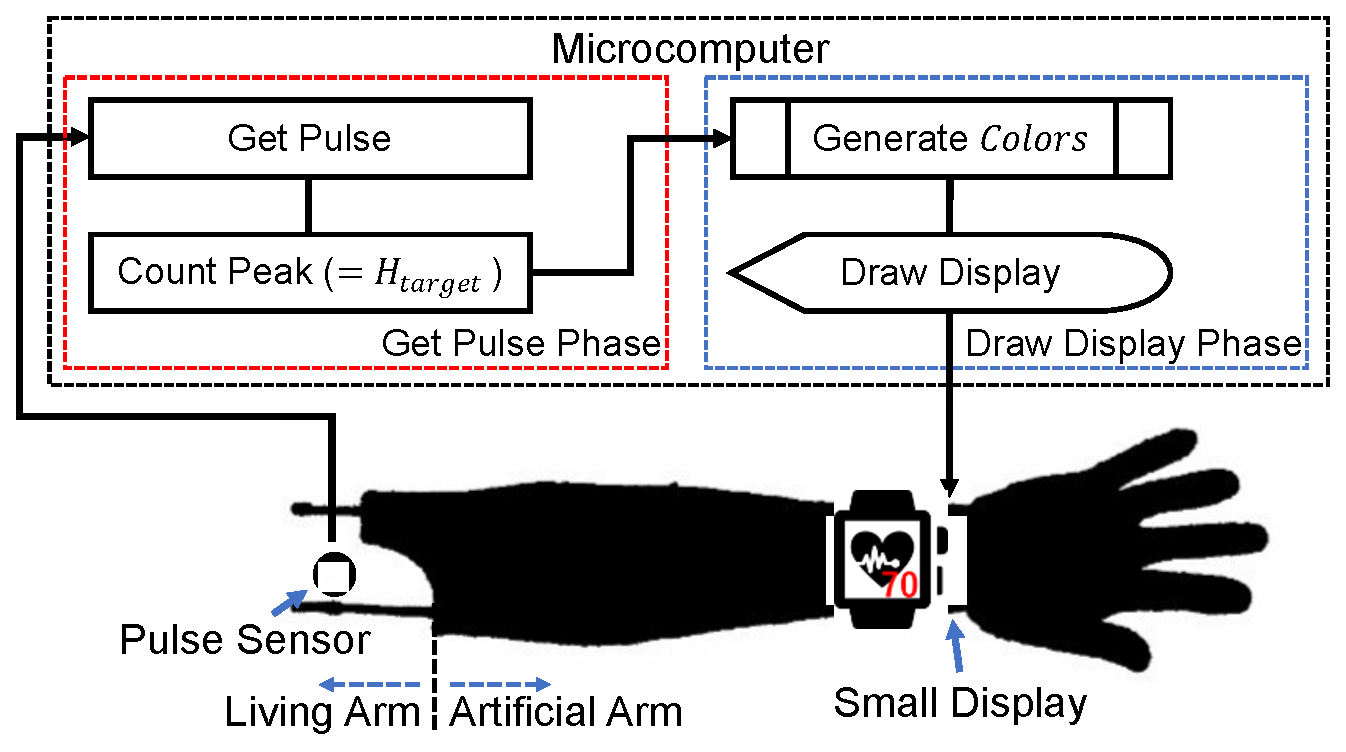
\includegraphics[width=1\linewidth]{method.eps}
  \end{center}
  \vspace{-8mm}
  \caption{提案システムの処理の流れ}
  \label{fig:method}
\end{figure}

\begin{table}[!t]
  \begin{center}
    \caption{識別精度の平均}
    \label{tab:result}
    \begin{tabular}{c|c} \hline\hline
    識別クラス数($C$) & 精度 \\ \hline
    10 & 0.649 \\
    2 & 0.976 \\ \hline
    \end{tabular}
  \end{center}
\end{table}

 \begin{thebibliography}{1}
 \bibitem{LiquidSense} Ren, Y., Tan, S., Zhang, L., Wang, Z., Wang, Z., and Yang, J.: Liquid Level Sensing Using Commodity WiFi in a Smart Home Environment, Vol. 4, No. 1, pp. 1--30 (2020).
 \end{thebibliography}
\end{document}